\fancychapter{Simulations}
\label{chap:sims}

    Simulations were used to validate the converter design and the \ac{mppt} algorithm before hardware implementation. This chapter presents the LTspice simulations of the photovoltaic model and the boost converter, an analytical power loss estimation in MATLAB, as well as the evaluation of the tracking algorithm in Simulink.

    \section{DC-DC Converter}

        The converter was simulated in LTspice to confirm the component selection under representative charging conditions. This section presents the photovoltaic cell model and the boost converter simulations used to compare inductor and capacitor options and to estimate ripple and efficiency.

    \subsection{Solar Panel model}

        The simulations started at LTspice with the aim to test the converter at different conditions. To achieve that, a \ac{pv} electrical model of the cells were designed using a five parameter model (1M5P) configuration. There are more electrical models that can simulate a solar panel, some with more accuracy but more complex. This model was perfect for the aim of the simulation since it is both reliable and simple.

        The 1M5P model represents the solar cell through a single diode equivalent circuit composed of a current source in parallel with one diode, a series resistance $R_s$, and a shunt (parallel) resistance $R_{sh}$, as shown in Figure~\ref{fig:pv_model}. The current source represents the photo generated current $I_{ph}$, which is proportional to the incident irradiance, while the diode accounts for the non linear $I$-$V$ characteristic of the p-n junction. The series resistance models the losses associated with the material bulk resistance, metal contacts and interconnections, whereas the shunt resistance represents the leakage currents through the cell, typically caused by manufacturing defects.

        The output current of the model is given by the characteristic equation~\ref{eq:1m5p}, where $I_0$ is the diode saturation current, $n$ is the diode identity factor, and $V_t$ is the thermal voltage \cite{LOBRANO2013894}. Together with $I_{ph}$, $R_s$ and $R_{sh}$, these constitute the five parameters that give the model its name.

        \begin{equation}
            I = I_{ph} - I_0 \left[ \exp\left(\frac{V + I R_s}{n V_t}\right) - 1 \right] - \frac{V + I R_s}{R_{sh}}
            \label{eq:1m5p}
        \end{equation}

        These parameters are not directly provided by manufacturers, but can be extracted from the standard datasheet values, namely the open-circuit voltage ($V_{oc}$), short-circuit current ($I_{sc}$), voltage and current at the \ac{mpp} ($V_{mp}$, $I_{mp}$), and the respective temperature coefficients, through a set of equations that ensure the model matches these reference points under Standard Test Conditions (STC). There are several ways to do it, however it is outside the range of this work. To simplify, calculations were carried using online tools and will not be explained in detailed here. 

        This approach allows the panel behavior to be accurately reproduced under different irradiance and temperature conditions, while keeping the circuit implementation simple enough to be integrated directly into LTspice.

        \begin{figure}[!ht]
            \centering
            
\includegraphics[width=0.9\textwidth]{Images/Implementation/PV model.png}
            \caption{Solar panel model diagram (1M5P configuration).}
            \label{fig:pv_model}
        \end{figure}
        
    \subsection{Boost Converter}
    \label{subsubsect:Sim_Boost}
        To validate the theoretical  calculations, simulations in LTspice were carried using the boost converter in steady state mode and a fix duty cycle. 

        Considering a solar panel with 35 cells, five points of CC-CV charging curve were chosen to test the performance of the converter. These five points are represented in Figure~\ref{fig:cc-cv points}.
        
        \begin{figure}[!ht]
            \centering
            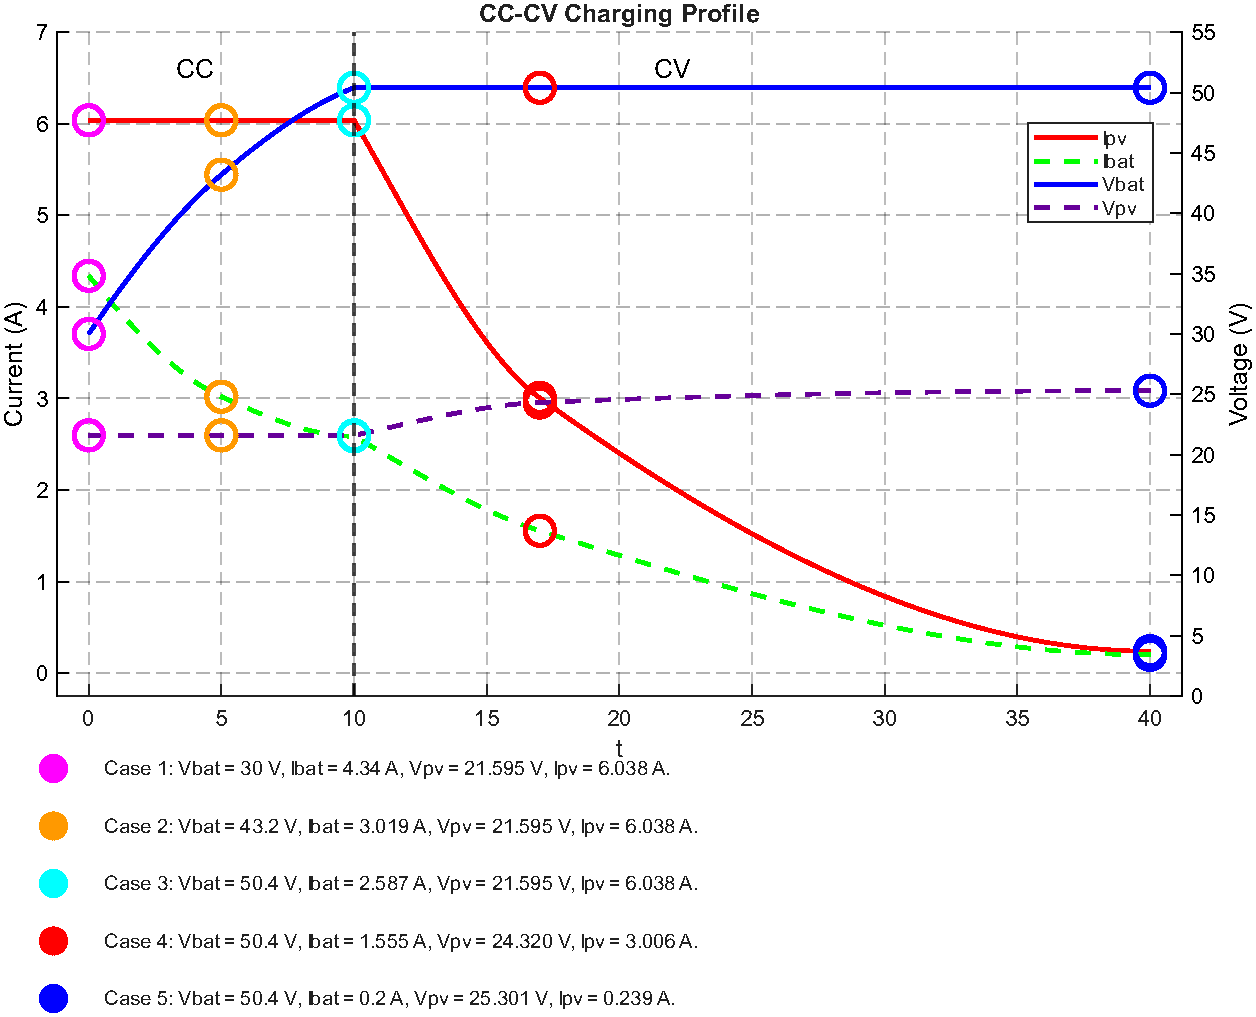
\includegraphics[width=0.9\textwidth]{Images/Implementation/cc_cv_points.pdf}
            \caption{CC-CV charge characteristics and analysis point selection.}
            \label{fig:cc-cv points}
        \end{figure}

        It is important to note that in this CC-CV curve the constant current is given by the solar panel and not by the battery as it is usually expected. This is only truth due to the maximum charge current of the battery being lower than the current that can be provided by the solar panel. So at CC, the converter is working at \ac{mpp}.

        With this five points chosen, some simulations were carried using capacitors and inductors that would fit the requirements calculated earlier. The objective of these simulations is to optimize the performance of the converter, leading to better choices.

        The model was built in LTspice with approximated models given by the manufactures for higher precision. Only the solar panel model was designed by hand, as previously mentioned.

        The battery was simulated using a voltage source and a resistor representing the internal resistance of the battery.

        The dead time of the transistors was implemented too. Using laboratory measurements, the rising and falling timing was measured and used in simulation. Has for the dead time, it is used the same as in the final prototype.

            \begin{figure}[!ht]
            \centering
            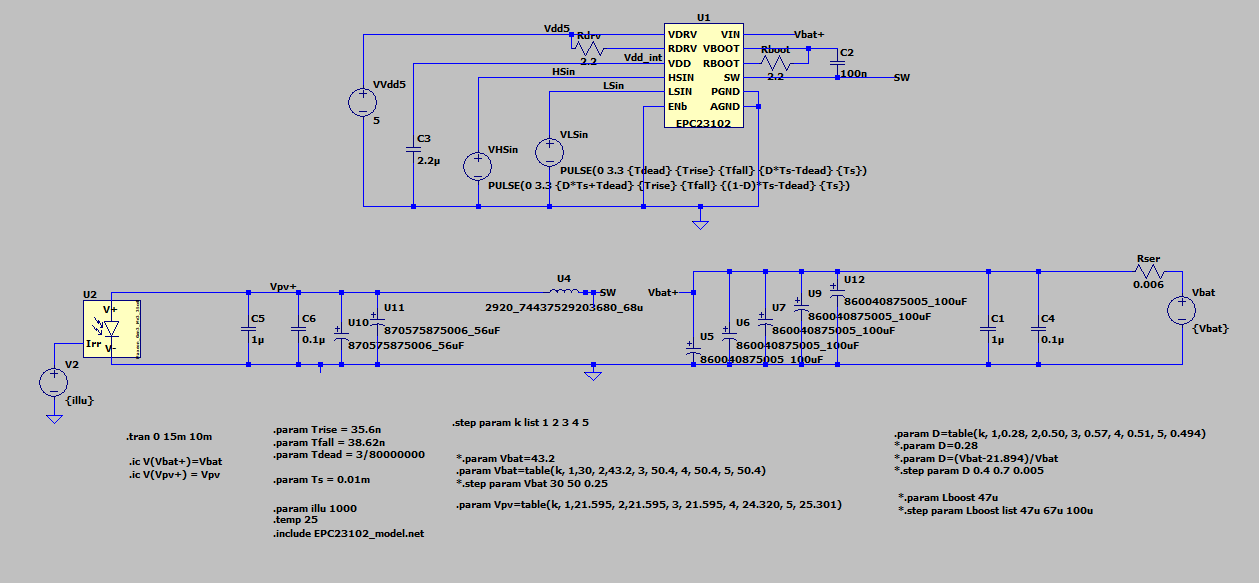
\includegraphics[width=0.9\textwidth]{Images/Implementation/Sim_circuit.png}
            \caption{Simulation circuit schematic.}
            \label{}
        \end{figure}


        The first simulations were carried to choose the input and output capacitors. The idea is to simulate the circuit using a known inductor (68~uH) and change the capacitors for different configurations. All configurations are overdimensioned to give low ripples (current and voltage). So the main factor is the efficiency of the converter.

        In Table~\ref{tab:loss_capacitors_2} is shown the results. The efficiency of all combinations are very high however the highest is the one with two 56~uF as input capacitors and tree 220~uF capacitors as output capacitors. Unfortunately the 220~uF were not available at the moment, so the second best option was chosen, the five 100~uF capacitors.

        It is worth noting that this is a simulation and therefore the efficiency is higher than what will be measured in laboratory results. Additionally, the difference between each combination it is very small. To make the product cheaper the third option would be as great as the one chosen.

        
        \begin{table}[!ht]
            \caption{Loss (\%) for different capacitor configurations (Cin, Cout).}
            \centering
            \begin{tabular}{|c|cccc|}
            \hline
            \textbf{Case \#} & \textbf{2x56 $\mu$F, 3x220 $\mu$F} & \textbf{100 $\mu$F, 3x220 $\mu$F} & \textbf{100 $\mu$F, 5x100 $\mu$F} & \textbf{2x56 $\mu$F, 5x100 $\mu$F} \\
            \hline
            1 & 0.5729 & 0.5796 & 0.5856 & 0.5788 \\
            2 & 0.6762 & 0.6985 & 0.7069 & 0.6844 \\
            3 & 0.7359 & 0.7655 & 0.7743 & 0.7449 \\
            4 & 0.6654 & 0.7091 & 0.7161 & 0.6735 \\
            5 & 3.4177 & 3.7148 & 3.7554 & 3.4671 \\
            \hline
            \end{tabular}
            
            \label{tab:loss_capacitors_2}
        \end{table}

        Similar to the previous simulation, the inductor was chosen by keeping all components with the same values (the capacitors used were Cin = 2x56uF and Cout = 5x100uF) and changing the inductor. Similar to before, all inductors simulated are within the minimum required.

        The losses for each case are represented in Table~\ref{tab:loss_inductance_2}. Similar to before, the efficiency difference is very low but not as linear as in the previous simulation, likely due to the inductor models chosen.

        The inductor chosen will highly influence the input ripple which can generate heat, and electrical interference. Table~\ref{tab:delta_iin_inductance} shows the different ripple currents for each inductor in each case of the CC-CV curve. The 22~uF inductor showed higher ripple current reaching values close to the input current. The inductor chosen was the 68~uF since it has overall good efficiency and reasonable input current ripple.


        \begin{table}[!ht]
            \caption{Loss (\%) for different inductance values.}
            \centering
            \begin{tabular}{|c|ccccc|}
            \hline
            \textbf{Case \#} & \textbf{22 $\mu$H} & \textbf{33 $\mu$H} & \textbf{47 $\mu$H} & \textbf{68 $\mu$H} & \textbf{100 $\mu$H} \\
            \hline
            1 & 0.4206 & 0.4439 & 0.5453 & 0.5788 & 1.2659 \\
            2 & 0.6645 & 0.6793 & 0.6627 & 0.6844 & 1.3664 \\
            3 & 0.7883 & 0.8076 & 0.7290 & 0.7449 & 1.4193 \\
            4 & 1.0556 & 1.0583 & 0.6867 & 0.6735 & 0.9624 \\
            5 & 6.7045 & 6.6230 & 3.6556 & 3.4671 & 3.8177 \\
            \hline
            \end{tabular}
            \label{tab:loss_inductance_2}
        \end{table}


        \begin{table}[!ht]
            \caption{$\Delta i_{L}$ ($I_{L,\max} - I_{L,\min}$) for different inductance values.}
            \centering
            \begin{tabular}{|c|ccccc|}
            \hline
            \textbf{Case \#} & \textbf{22 $\mu$H} & \textbf{33 $\mu$H} & \textbf{47 $\mu$H} & \textbf{68 $\mu$H} & \textbf{100 $\mu$H} \\
            \hline
            1 & 2.6939 & 1.8906 & 1.3256 & 0.9781 & 0.6251 \\
            2 & 4.7934 & 3.3416 & 2.3354 & 1.7066 & 1.0707 \\
            3 & 5.4733 & 3.8253 & 2.6813 & 1.9644 & 1.2839 \\
            4 & 5.5596 & 3.8565 & 2.7075 & 2.0139 & 1.2925 \\
            5 & 5.5520 & 3.8510 & 2.6903 & 1.9636 & 1.2344 \\
            \hline
            \end{tabular}
            \label{tab:delta_iin_inductance}
        \end{table}

        Now that the converter components are all chosen, the following measurements were taken in LTspice:

        \begin{table}[!ht]
        \centering
        \caption{Ripple and Power Loss Summary for Each Operating Step}
        \label{tab:ripple_loss}
        \begin{tabular}{|c|cccc|}
        \hline
        \textbf{Case \#} & \textbf{$\Delta V_{bat}$ (V)} & \textbf{$\Delta V_{pv}$ (V)} & \textbf{$\Delta I_{L}$ (A)} & \textbf{Loss (\%)} \\
        \hline
        1 & 0.0406 & 0.0145 & 0.9781 & 0.578 \\
        2 & 0.0491 & 0.0212 & 1.7066 & 0.684 \\
        3 & 0.0529 & 0.0244 & 1.9644 & 0.745 \\
        4 & 0.0406 & 0.0220 & 2.0139 & 0.674 \\
        5 & 0.0302 & 0.0215 & 1.9636 & 3.464 \\
        \hline
        \end{tabular}
        \end{table}

        \textcolor{red}{Iin é difrente de IL. O Iin tem quase nada de ripple}


        Both voltage ripples are lower than what was defined as the goal in Table~\ref{tab:converter_constraints}. As for the current ripple it is still reasonable. The losses/efficiency are also higher than what was aimed, reaching values up to 99.4\%, in simulation. 

        A voltage sweep were performed, and as expected the efficiency drop with the increase of output voltage (Figure~\ref{fig:voltage_sweep}). Also, as mentioned earlier, the output current drop because in \ac{cc} mode the solar panel current is constant, so the output current drops with the increase of battery voltage due to the power conservation principle.

        \begin{figure}[!ht]
            \centering
            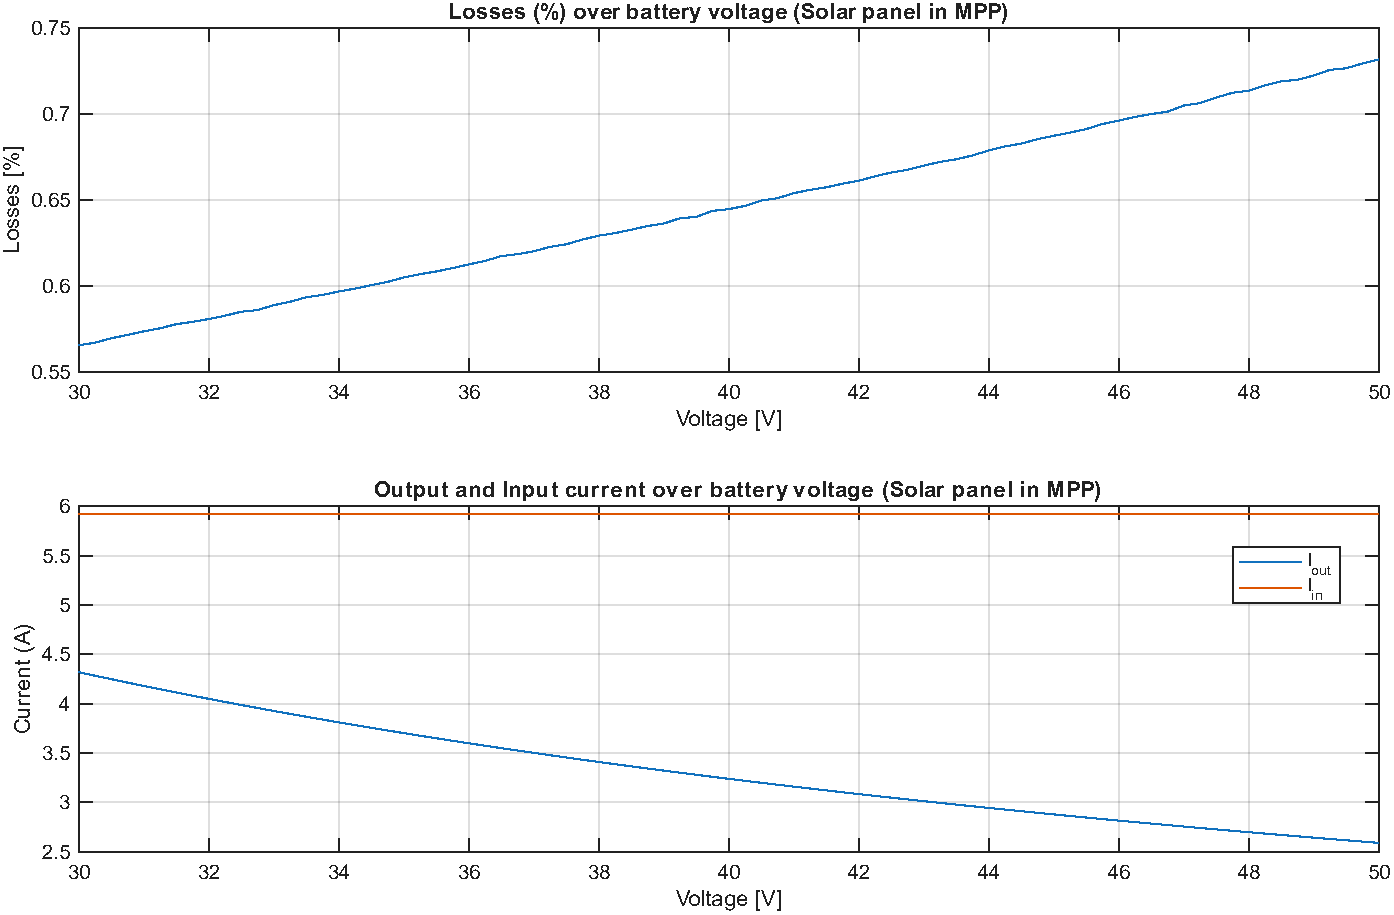
\includegraphics[width=0.7\textwidth]{Images/Implementation/vbat__sweep_sim_res.pdf}
            \caption{Battery voltage sweep simulation results.}
            \label{fig:voltage_sweep}
        \end{figure}

        Note: in version 1.1 of the prototype it was added two shotcky diodes that were not considered in these simulations. The diodes slightly increase the efficiency of the converter (+0.03\%) due to their lower forward voltage. The increase could be higher if the dead time was longer. Since the dead time is only 0.375~\% of the PWM period, the difference is negligible and therefore its use is irrelevant.

    \section{Power Loss Estimation}
        \label{subsubsec:loss_estimation}

        Although LTspice provides an accurate estimation of the converter efficiency, it does not directly identify the contribution of each component to the total power dissipation. Therefore, an analytical power loss model was developed in MATLAB to estimate the individual losses of each component of the proposed synchronous boost converter. The model uses the electrical parameters of the selected components obtained from their datasheets together with the converter operating conditions.

        The total converter losses are obtained by summing the losses associated with the GaN transistors, inductor, capacitors, dead time and gate driver:

        \begin{equation}
        P_{loss}=P_{cond_{HS}}+P_{cond_{LS}}+P_{sw_{HS}}+P_{sw_{LS}}+P_{L}+P_{C}+P_{dead}+P_{gate}.
        \end{equation}

        \textcolor{red}{falta coisas}
        The converter efficiency is then calculated as:

        \begin{equation}
        \eta=\frac{P_{out}}{P_{out}+P_{loss}}\times100\%.
        \end{equation}

        The conduction losses of each GaN transistor are given by:

        \begin{equation}
        P_{cond}=I_{RMS}^{2}R_{DS(on)}.
        \end{equation}

        These losses are primarily caused by the on state resistance of the transistors, resulting in power dissipation whenever current flows through the channel. 

        The switching losses are estimated using Equation~\ref{eq:psw}, 
        which takes into account the loses during the period when the transistor is not fully on nor fully off. Also, the losses associated with charging and discharging the output capacitance of each transistor.

        \begin{equation}
        P_{sw}=\frac{1}{2}V_{out}I_{L_{AVG}}(t_r+t_f)f_{sw} + \frac{1}{2}C_{oss}V_{out}^{2}f_{sw}
        \label{eq:psw}
        \end{equation}

        The dead-time losses are calculated using Equation~\ref{eq:pdead}. These losses originate from the conduction of the reverse conduction path during the dead time interval required to prevent shoot through. This reverse condition path is either from the third quadrant conduction from the GaN device or from the parallel schottky diode added later in version 1.1 (this is explained in Section \textcolor{red}{?})

        \begin{equation}
        P_{dead}=2\cdot  V_f \cdot I_{L_{AVG}} \cdot t_{dead} \cdot f_{sw}.
        \label{eq:pdead}
        \end{equation}



        The inductor and \ac{dc} capacitor losses are estimated using the RMS current passing through them and their \ac{esr}

        \begin{equation}
        P_L=I_{L_{RMS}}^{2}ESR.
        \end{equation}

        \begin{equation}
        P_C=I_{C_{RMS}}^{2}ESR,
        \end{equation}

        Although magnetic core losses of the inductor could be estimated too, the selected manufacturer does not provide the required magnetic material parameters. Consequently, only the winding copper losses are considered, leading to a slight underestimation of the total converter losses. 

        \textcolor{red}{reler o texto, inserir as perdas do circuito auxiliar, inserir as perdas vindas do REDEEXPERT, adicionar as perdas vinda do sensor de corrente, simplificar ou não a pie chart}

        Finally, the gate driver losses are estimated using Equation~\ref{eq:gate_drive} which takes into account the energy needed to drive the transistors. Although the EPC23102 has an internal gate driver, this is still relevant.

        \begin{equation}
        P_{gate}= (Qg_{LS} + Qg_{HS})* Vdrv * fsw.
        \label{eq:gate_drive}
        \end{equation}

        Figure~\ref{fig:loss_breakdown} presents the resulting power loss distribution. The calculated total power loss is approximately 1.188~W, corresponding to an efficiency of 99.10\%, which agrees well with the LTspice simulation results presented in the previous section.

        \begin{figure}[!ht]
            \centering
            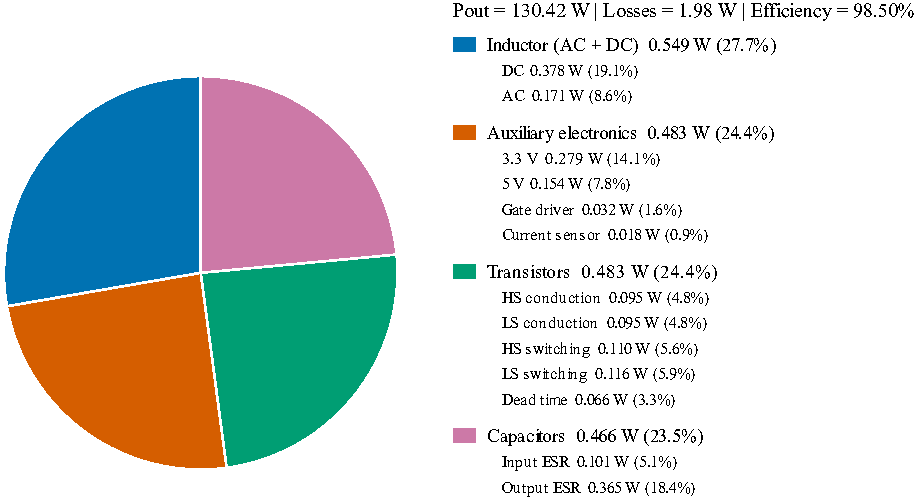
\includegraphics[width=0.9\textwidth]{Images/Implementation/fig_loss_breakdown.pdf}
            \caption{Analytical power loss distribution of the synchronous boost converter for Case~1. \textcolor{red}{change for the case 2}}
            \label{fig:loss_breakdown}
        \end{figure}

        The largest contributors to the total losses are the inductor copper losses and the capacitor ESR losses, each accounting for approximately 31.5\% of the total power dissipation. This highlights the importance of selecting an inductor with low winding resistance and capacitors with low ESR, as these passive components dominate the converter losses.

        The conduction losses of the GaN transistors account for approximately 16\% of the total losses, showing the importance of choosing transistors with low conduction resistance. The high-side device dissipating more power than the low-side transistor due to its longer conduction interval. Switching losses represent approximately 12\% of the total losses, including both transition losses and the energy required to charge and discharge the output capacitances. Dead-time losses contribute approximately 7\%, while the gate driver losses are almost negligible (only 2.7\%).

        Additionally, all \ac{pcb} connections have an inductance that will represent losses too. 

        Overall, the analysis indicates that nearly two-thirds of the converter losses originate from the passive components, whereas the semiconductor devices account for approximately one-third. It should be noted that the presented values are based on analytical equations and datasheet parameters. Since magnetic core losses were not considered, the calculated efficiency represents a slight overestimation of the actual converter performance.

        However, both simulation and theoretical analysis indicate that the choice of each components lead to a highly efficient converter.

    \section{MPPT algorithm}
        The algorithm has a few parameters like the working frequency, sampling frequency, step size, power dead band, etc. All of this parameters need to be tuned to work on his full potential while keeping it safe. Therefore, a simulation in MATLAB Simulink was implemented which simulates the behavior of the switching converter with the values defined earlier. The boost converter is connected to a solar panel and a battery, as it is spouse to be use (Figure~\ref{fig:Simulink mode}). To simplify, the simulation uses a diode instead of a transistor making it a basic boost converter. This simplification will not have influence on the results since the idea is to analyze the performance of the algorithm instead of the converter efficiency.

        \begin{figure}[!ht]
            \centering
            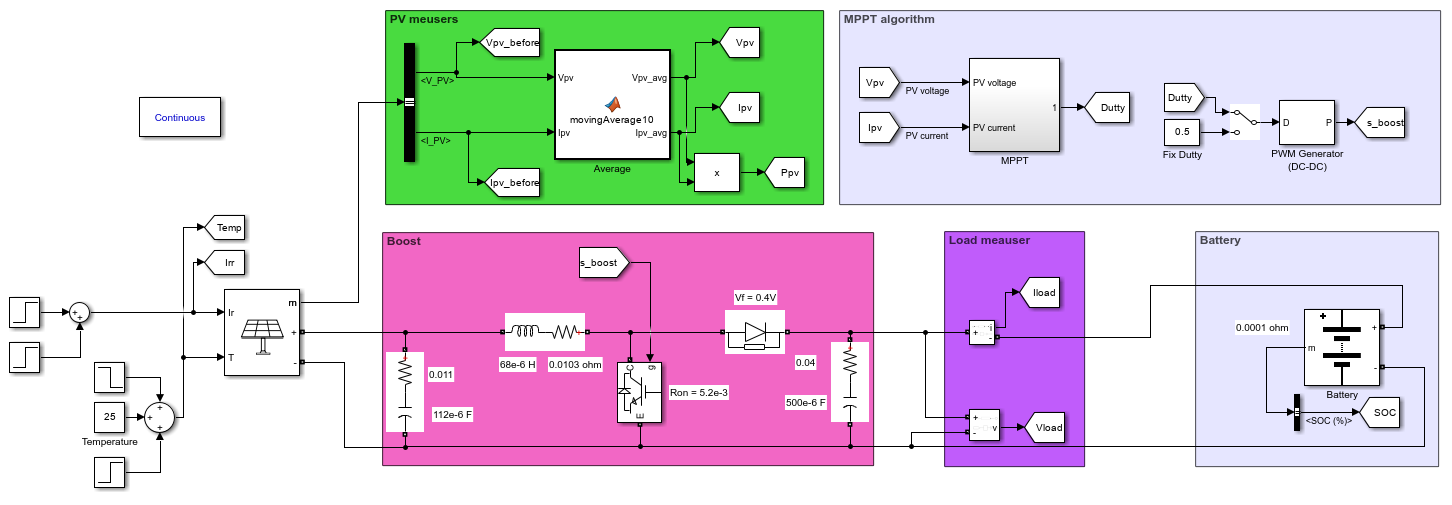
\includegraphics[width=0.9\textwidth]{Images/Implementation/simulink_sim.png}
            \caption{MATLAB Simulink MPPT simulation model.}
            \label{fig:Simulink mode}
        \end{figure}

        The solar panel and battery are both configured with the parameters of the real system. It was used the specifications of solar panel with 35 cells and the \ac{sg01} battery. The \ac{pv} side sensors are inside the solar panel and show some noise as in the real system, to mitigate it, an average of 10 samples was implemented with each sample collected at 1~KHz. The value of the average is sent to the algorithm which runs at 100~Hz. Inside the \ac{mppt} block are the sweep algorithm and \ac{peo}.

        To understand the impact of each environment variation on the \ac{mpp} point, a sweep  was performed for different irradiance values and temperatures, Figure~\ref{fig:irr_sweep} and \ref{fig:temp_sweep}. For irradiance variations, the maximum duty cycle difference is 3\%. On the other hand, the maximum duty cycle difference for temperature variations is 9\%. This means that the algorithm will always be slower to temperature variations when compared to irradiance variations. However, it is more common to have a fast changing irradiance than temperature. The solar panels will heat slowly and when covered in water they cool around 10 to 20ºC (values measured during tests).  

        \begin{figure}[!ht]
            \centering
            \begin{minipage}[b]{0.49\textwidth}
                \centering
                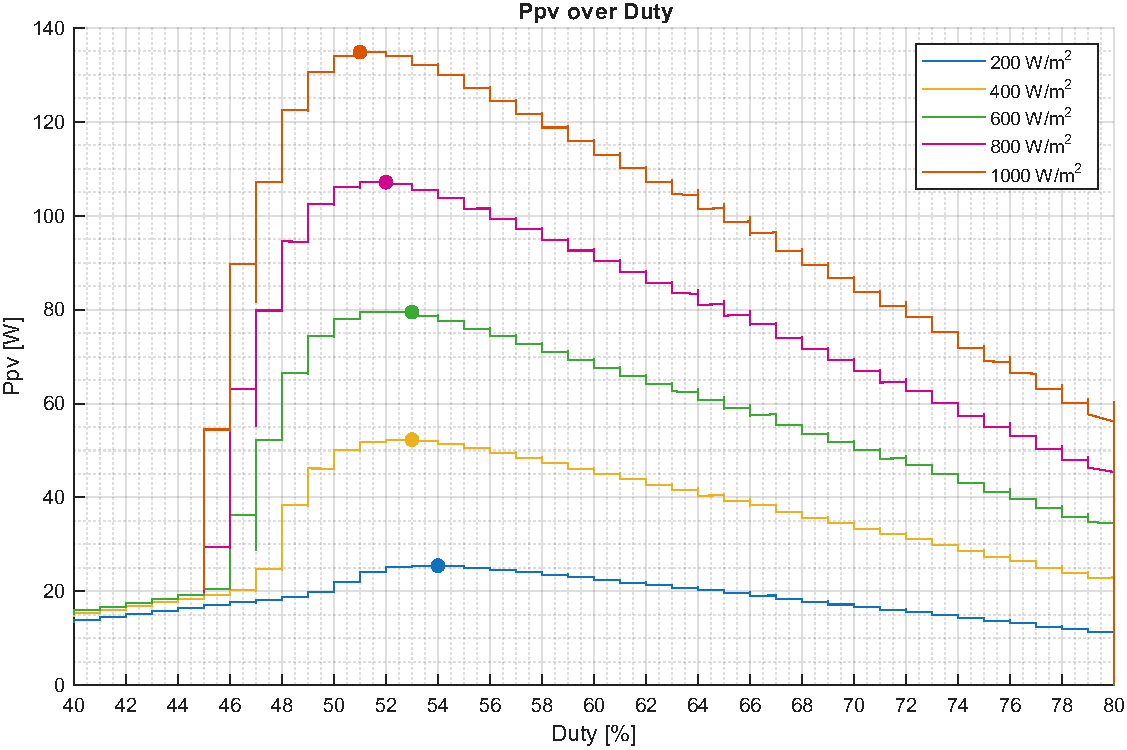
\includegraphics[width=\textwidth]{Images/LAB_res/sweep_duty_irr.pdf}
                \caption{Duty cycle sweep with different values of irradiance.}
                \label{fig:irr_sweep}
            \end{minipage}
            \hfill
            \begin{minipage}[b]{0.49\textwidth}
                \centering
                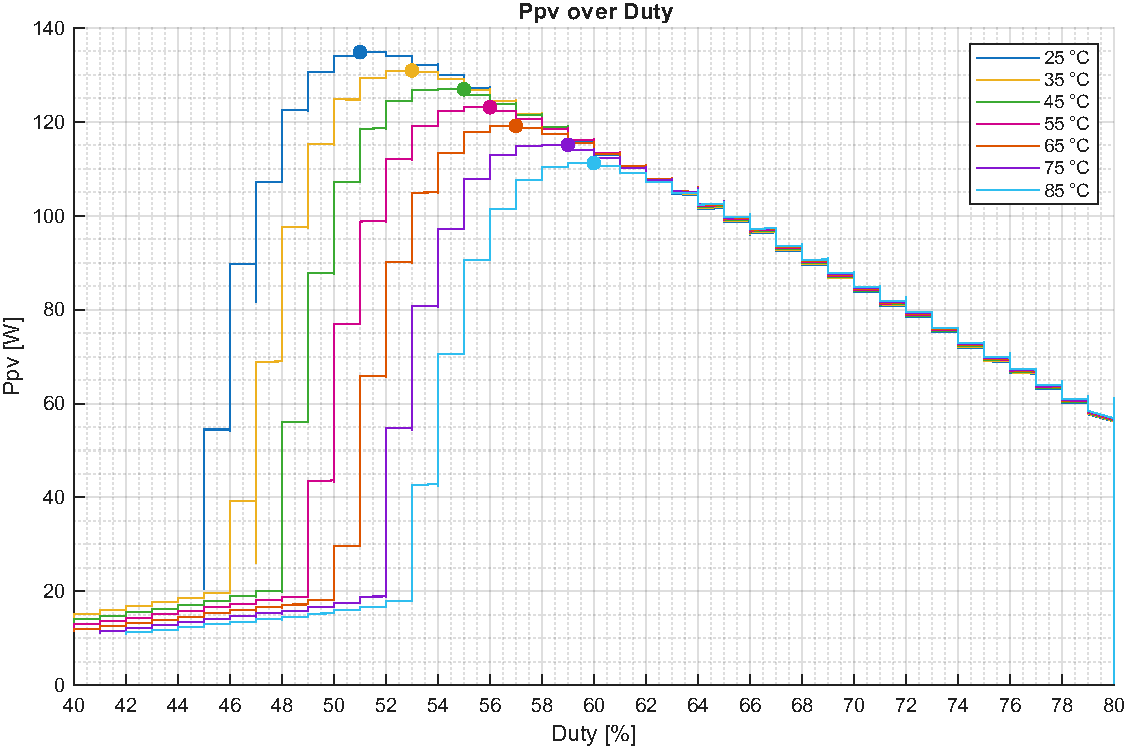
\includegraphics[width=\textwidth]{Images/LAB_res/sweep_duty_temp.pdf}
                \caption{Duty cycle sweep with different values of temperature.}
                \label{fig:temp_sweep}
            \end{minipage}
        \end{figure}

        Let's consider the worst case which is 9\%. To achieve the desired speed of 0.5~seconds, a combination of the step size and working frequency needs to be tuned. For example, considering a working frequency of 100~Hz, the algorithm have 50 steps to achieve \ac{mpp} under 0.5 seconds. So if the algorithm uses a step size of 9\% divided by 50 (0.18\%), in an ideal situation it would reach the speed goal every time. However, since this is a small step it can be confused with noise. Therefore, always needs to be tuned to the systems where is being applied.

        In simulations, the system can be tested with different parameters to give an idea of how it should behave outside simulation. Fixing the frequency to 100~Hz, a simulation was performed with 3 different step sizes under a few steps of temperature, Figure~\ref{fig:peo_step_comparison}. The smaller step is too small, and therefore it never reaches the \ac{mpp}. Most likely due to the noise. The other two show a similar performed, but the higher step show more oscillations around the \ac{mpp}.


        \begin{figure}[!ht]
            \centering

            \begin{subfigure}[b]{0.49\textwidth}
                \centering
                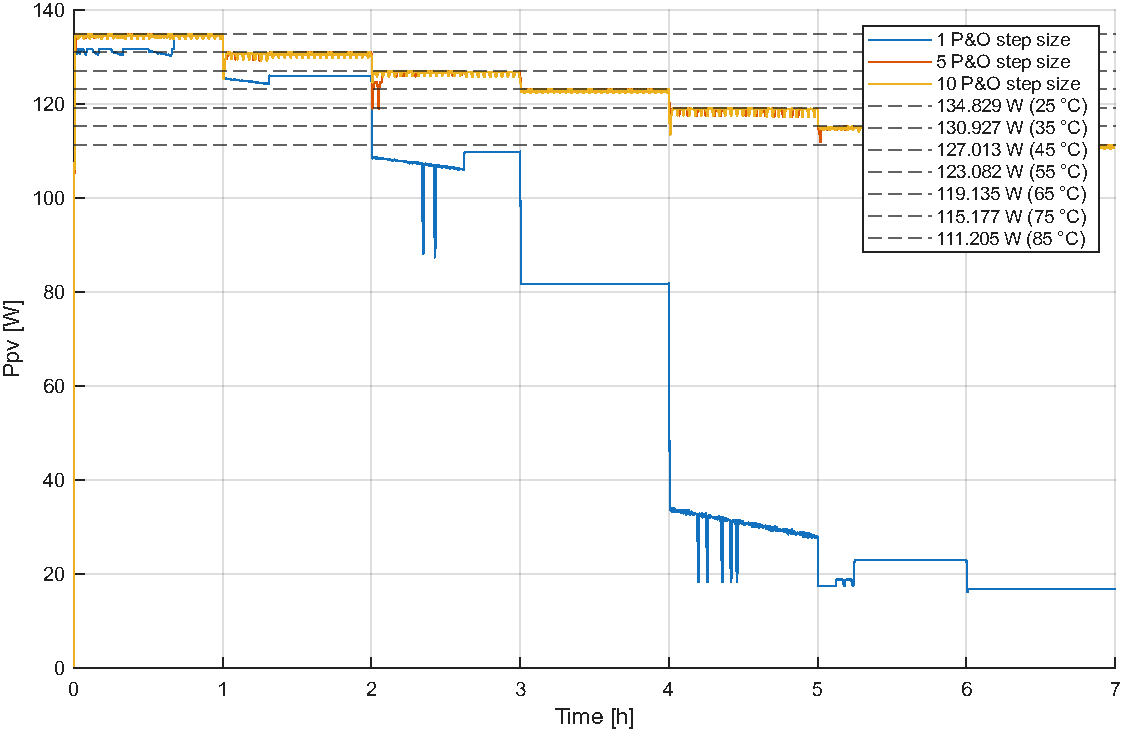
\includegraphics[width=\textwidth]{Images/Implementation/Tracking_speed_PEO_step2}
                \caption{Complete response.}
                \label{fig:peo_step_complete}
            \end{subfigure}
            \hfill
            \begin{subfigure}[b]{0.49\textwidth}
                \centering
                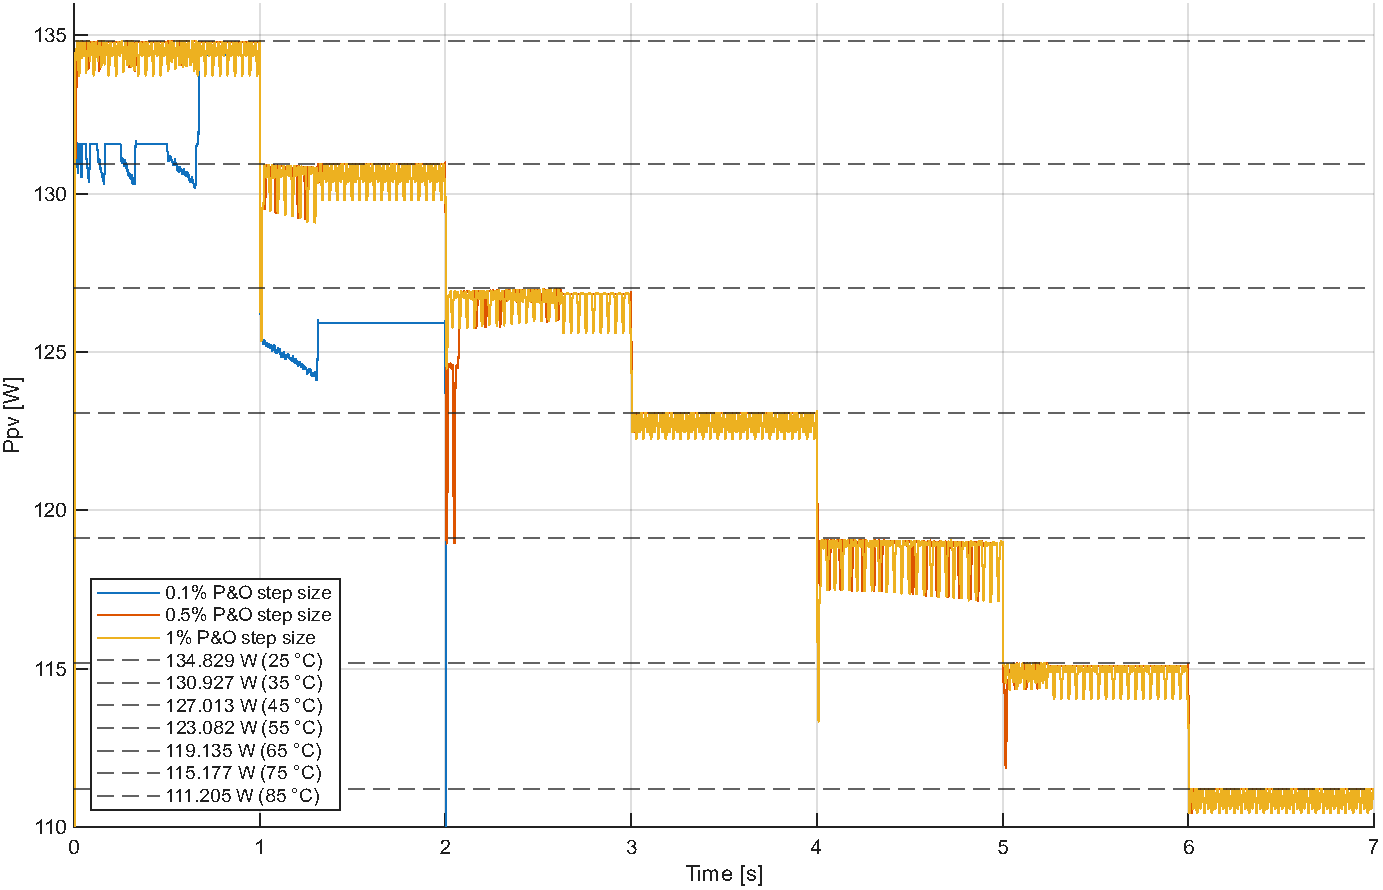
\includegraphics[width=\textwidth]{Images/Implementation/Tracking_speed_PEO_step.pdf}
                \caption{Zoomed view.}
                \label{fig:peo_step_zoom}
            \end{subfigure}

            \caption{Power response for different \ac{peo} step sizes during a temperature variation of $10\,^{\circ}\mathrm{C}$ per second.}
            \label{fig:peo_step_comparison}
        \end{figure}

        The analysis was then extended to more severe operating point variations. For a temperature step from $25~^\circ\mathrm{C}$ to $85~^\circ\mathrm{C}$ (Figure~\ref{fig:big_temp_step}), the $0.5\%$ duty-cycle step, which had performed well in the previous test, required the longest tracking time, approximately $1~\mathrm{s}$ to reach within $5\%$ of the \ac{mpp}. Given that the tracking time requirement is at most $1~\mathrm{s}$, and typically below $0.5~\mathrm{s}$, this step size lies at the limit of the specification. The $1\%$ and $2\%$ steps reached the \ac{mpp} faster, but with larger oscillations around the operating point. A step size between $0.5\%$ and $1\%$ is therefore considered the most suitable compromise.

        It should also be noted that the algorithm stalled on a few occasions. This behavior is attributed to measurement noise and to the \ac{peo} deadband. Although not desirable, it is consistent with the expected operation of the method and can be reduced by further tuning.

        A rapid irradiance variation was also simulated. As shown in Figure~\ref{fig:big_irr_step}, the \ac{mpp} is reached almost instantaneously for all step sizes under consideration. This result is expected, as discussed earlier, since the corresponding duty cycle variation is approximately three times smaller than in the temperature case.

        \begin{figure}[!ht]
            \centering
            \begin{minipage}[b]{0.49\textwidth}
                \centering
                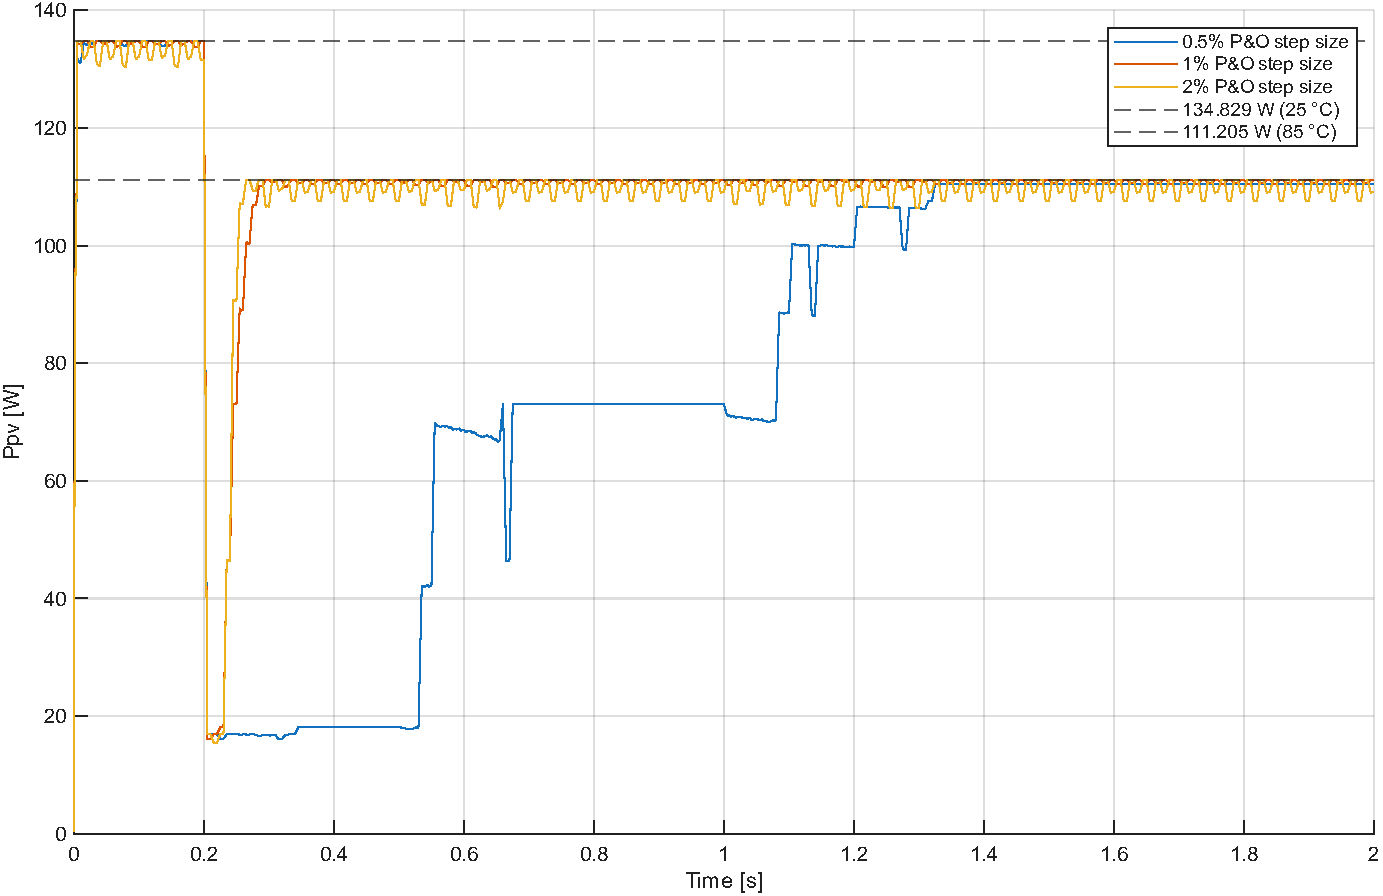
\includegraphics[width=\textwidth]{Images/Implementation/temp_step_PEOsteps.pdf}
                \caption{Power response for different \ac{peo} step sizes during a temperature variation from 25ºC to 85ºC.}
                \label{fig:big_temp_step}
            \end{minipage}
            \hfill
            \begin{minipage}[b]{0.49\textwidth}
                \centering
                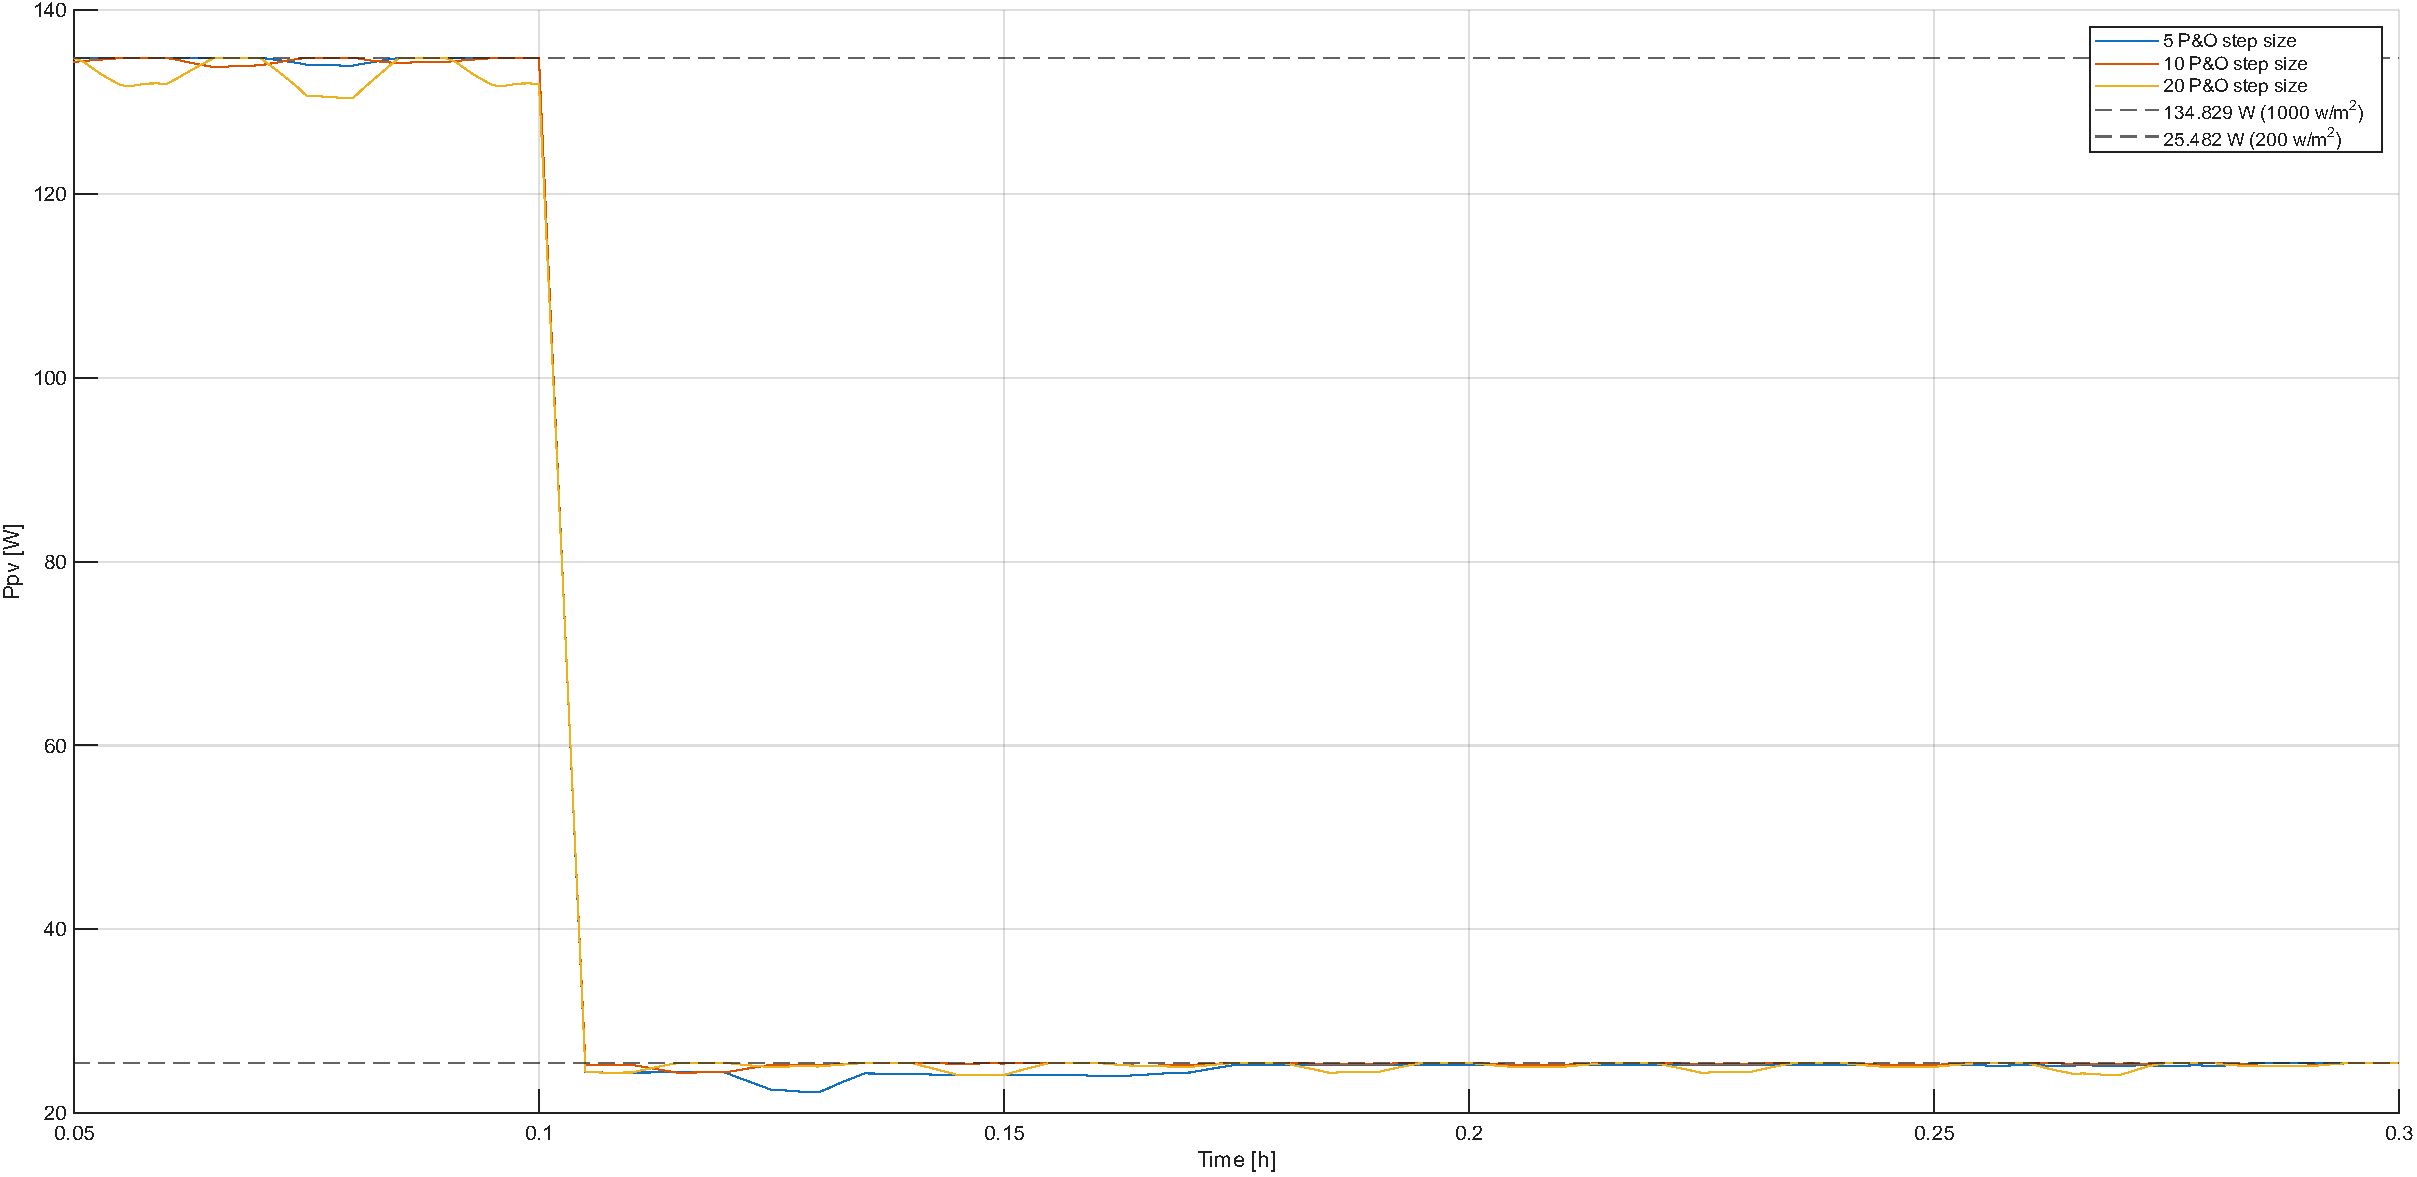
\includegraphics[width=\textwidth]{Images/Implementation/Irr_step_PEOsteps.pdf}
                \caption{Power response for different \ac{peo} step sizes during a Irradiance variation from 1000~$\mathrm{W/m}^2$ to 200~$\mathrm{W/m}^2$.}
                \label{fig:big_irr_step}
            \end{minipage}
        \end{figure}